\subsubsection{\p0d Energy Loss Correction}
\label{sec:Systematics_P0DELoss}

For tracks that begin in the \p0d and enter the TPC, there is an additional 
\p0d energy loss systematic effect that we needed to understand.  Currently, the
only way we can reconstruct the energy of \p0d tracks is to use the reconstructed
energy from the
Tracker momentum and add on an additional energy shift to correct for the \p0d energy loss.  
As such, there are two primary areas of concern: 1) How well does the MC simulate
the energy loss of the particle as it travels through the \p0d?  2) How well does
the current code reconstruct the energy loss in the \p0d?  Since the reconstruction
applied to Data and MC are the same, we decided that the second point would not
contribute to a difference between Data and MC, and that all differences between 
Data and MC would be due entirely to the first point.

To study this simulation systematic, we decided to look at muon-like tracks that
begin in the \p0d and enter TPC1.  By comparing the Data and MC TPC1 momentum 
distributions of tracks beginning at different \p0dules we were able to extract 
a simulation dependent effect along the z-axis (Figure \ref{fig:TPC1Mom_Compare}
).  In this way, the average TPC1 momentum difference between Data and MC is plotted
as a function of z for both water in and water out (Figure \ref{fig:TPC1Mom_AvgDiff}), 
with the maximum momentum cutoff set at 5 GeV.  This was chosen because at higher
energies, low statistics in the Data (in comparison with MC) skews the differences.
The linear fit gave the \p0d energy simulation systematic effect. In order to see 
how $\frac{N_{Data}}{N_{MC}}$ is affected by this energy loss systematic
we shifted the MC momentum using the fit data, according to each track's Z position,
and then recounted the $N_{MC}$ above and below 2 GeV.  The results are listed
in Table \ref{tab:EnergyLossSystematic}.

\begin{figure}
\centering
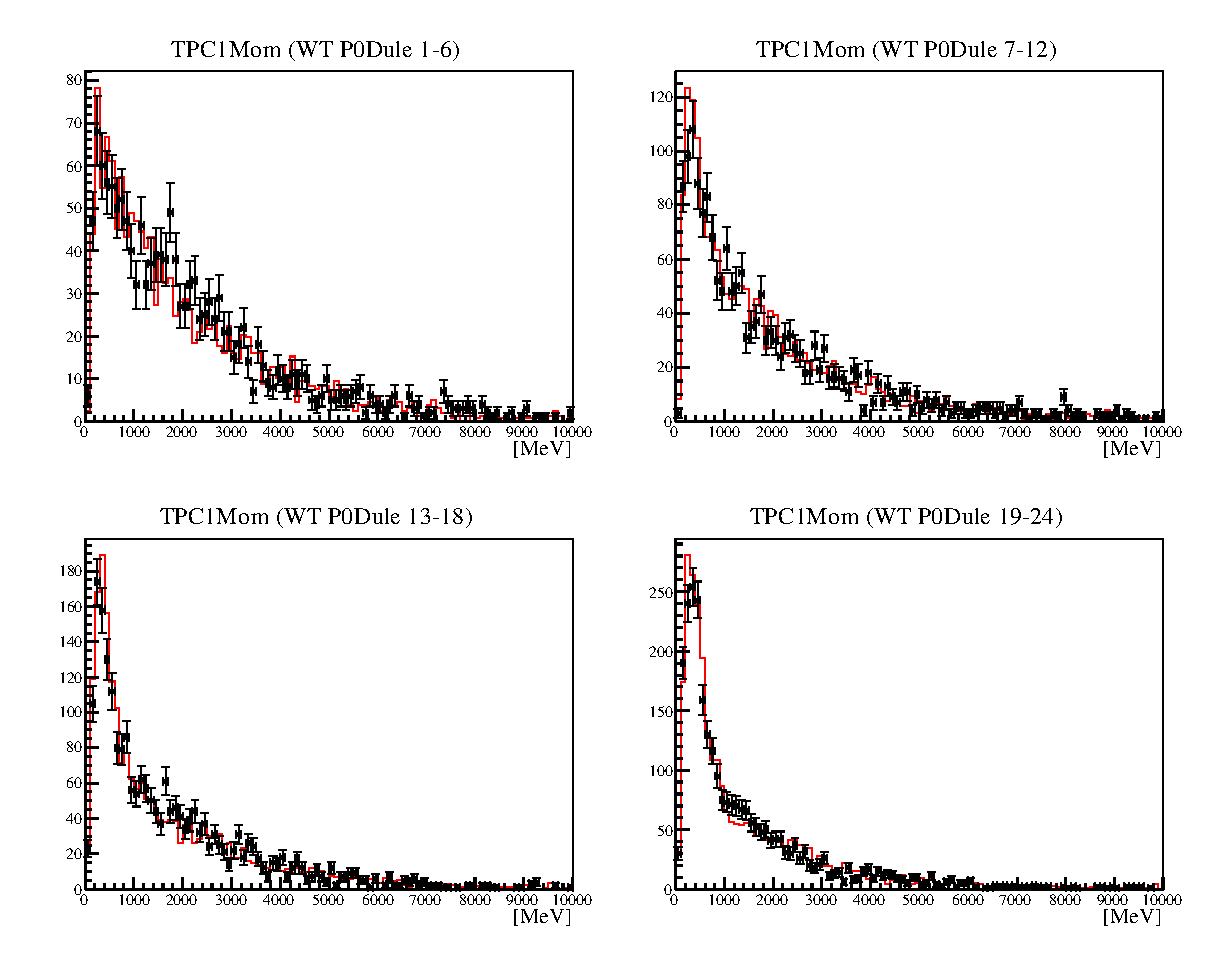
\includegraphics[width=5.5in]{Figures/TPC1Mom_Compare1.eps}
\caption{A sample selection of TPC1 momentum plotted for data (black) and MC (red)
starting in different WT \p0dules. Good agreement is observed} 
\label{fig:TPC1Mom_Compare}
\end{figure}

\begin{figure}
\centering
\subfloat[Run 1]{\label{fig:AvgDiff_run1}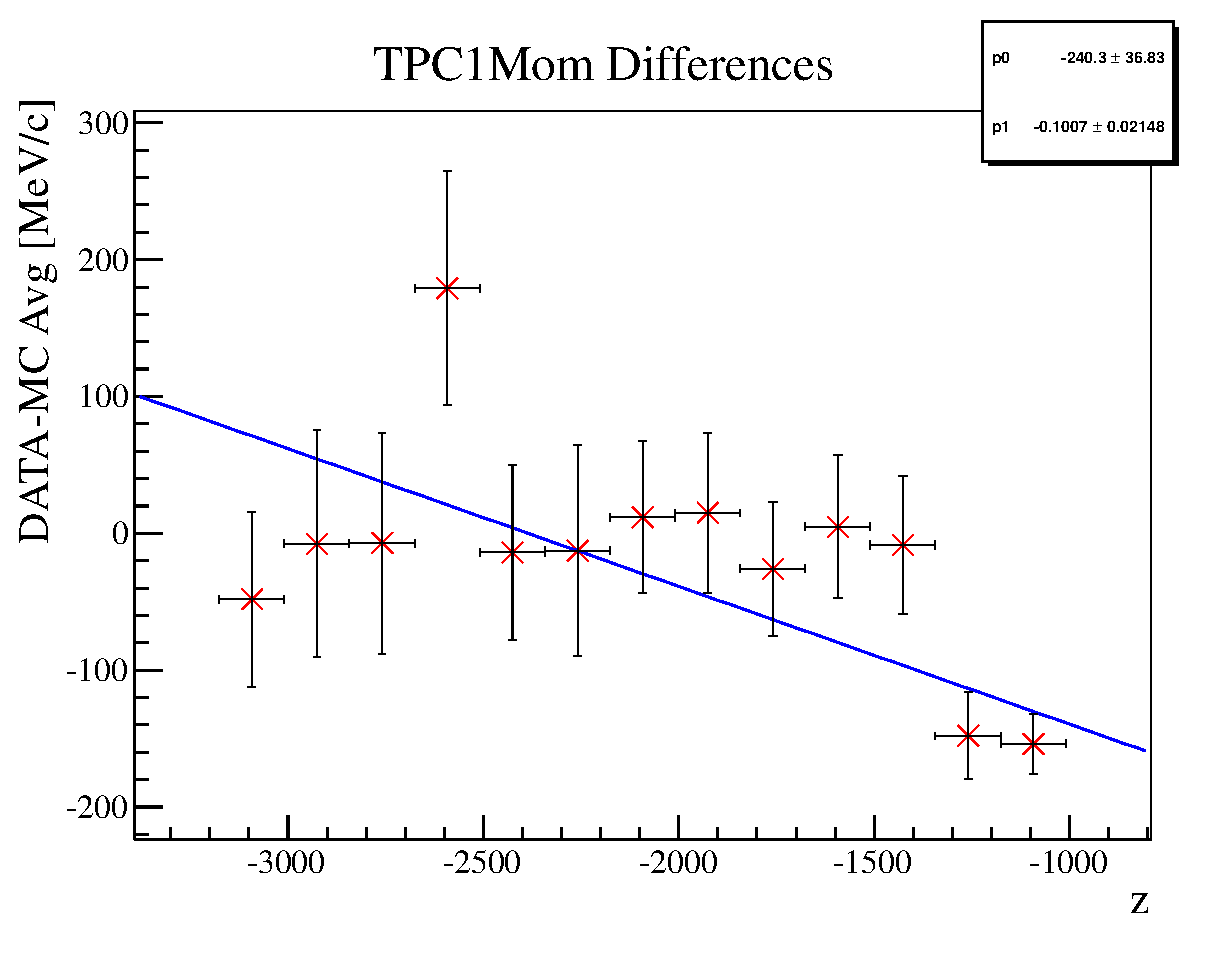
\includegraphics[width=3in]{Figures/AvgDiff_run1.eps}}
\subfloat[Run 2 Water]{\label{fig:AvgDiff_run2water}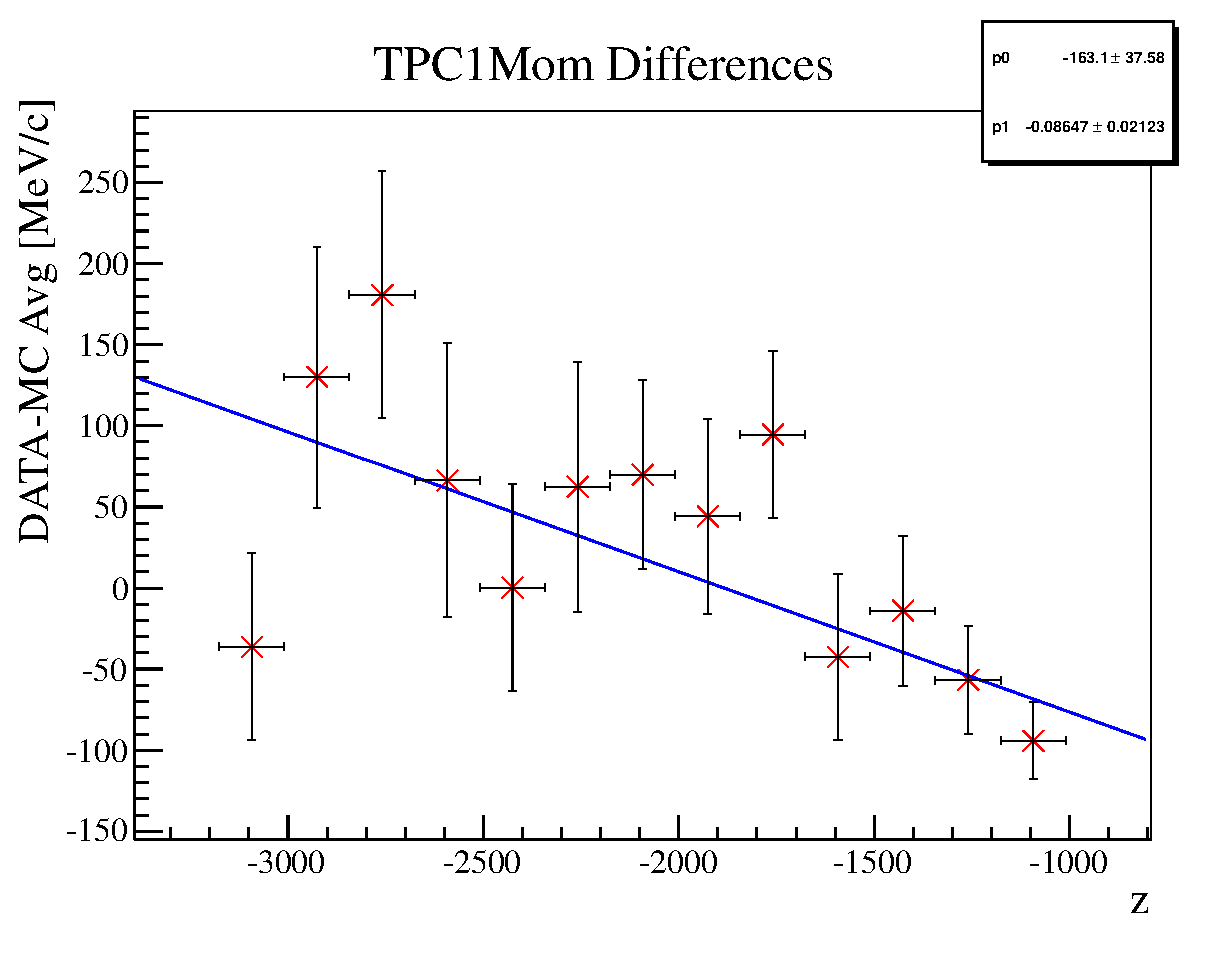
\includegraphics[width=3in]{Figures/AvgDiff_run2water.eps}}
\caption{Run 1 and Run 2 Water average TPC1 momenta differences between Data and MC, plotted for different
WT \p0dules} 
\label{fig:TPC1Mom_AvgDiff}
\end{figure}

\begin{table}
\caption{Systematic effect due to \p0d energy loss simulation effects.}
\label{tab:EnergyLossSystematic}
\centering
\begin{tabular}{rccc}\toprule
 & \multicolumn{2}{c}{$N_{\text{Data}}/N_{MC}$} \\ \cmidrule{2-3}
 &  Original & Adjusted & \% Difference\\ \midrule
 % Run 1   & 0.878 & 0.892 & 1.513 \\ 
 % Run 2 Water & 1.016 & 1.015 & -0.163 \\ 
 Run 1 (0-2 GeV)  & 1.023 & 1.016 & -0.743 \\ 
 Run 1 (2-5 GeV)  & 0.981 & 0.999 & 1.826 \\ 
 Run 1 (5+ GeV)  & 0.878 & 0.887 & 0.957 \\ 
 Run 2 Water (0-2 GeV)  & 1.013 & 1.015 & 0.135 \\ 
 Run 2 Water (2-5 GeV)  & 1.001 & 1.000 & -0.086 \\ 
 Run 2 Water (5+ GeV)  & 0.925 & 0.919 & -0.673 \\ 

\bottomrule
\end{tabular} 
\end{table}

